%\documentclass[prb.11pt,notitlepage]{revtex4-1}
%\documentclass[11pt,notitlepage]{revtex4-1}
\documentclass[11pt,a4paper]{article}
%---------------------------
% preambulo:
%---------------------------
\usepackage{abstract}
\usepackage[affil-it]{authblk}
\usepackage[utf8]{inputenc}	% encoding do arquivo, reconhecimento de acentos, etc.
\usepackage[brazilian]{babel}    % hiphenação em portugues
\usepackage{textcomp} % pacote para simbolos gregos no texto, sem ficar itálico
\usepackage{amsmath}    % need for subequations
\usepackage{amssymb}    % need for math symbols
\usepackage{graphicx}   % need for figures
\usepackage{verbatim}   % useful for program listings
\usepackage{color}      % use if color is used in text
\usepackage{subfigure}  % use for side-by-side figures
\usepackage{siunitx}
\usepackage{hyperref}   % use for hypertext links, including those to external documents and URLs
\usepackage[yyyymmdd,hhmmss]{datetime} % pacote para escrever a data de hoje
\usepackage[brazilian,nameinlink]{cleveref} % pacote para referenciar figuras e equacoes
\usepackage[table,xcdraw]{xcolor} % tabelas coloridas
\usepackage{circuitikz} %Pacote para desenhar circuitos
\usepackage{tikz}
\ctikzset{bipoles/length=0.9 cm} % tamanho dos componentes desenhados nos circuitos pelo pacote Circuitikz
\raggedbottom           % don't add extra vertical space
%---------------------------
%MARGENS
%---------------------------
\usepackage{indentfirst}        % indenta primeiro parágrafo
\setlength{\topmargin}{-15pt} % extra vert. space + at the top of header: 23pt
\setlength{\oddsidemargin}{-15pt} % extra spc added at the left of odd page: 0pt
\setlength{\textheight}{625pt} % comprimento do corpo do texto
\setlength{\textwidth}{480pt} % largura do corpo do texto
\setlength{\footskip}{50pt} % distancia da ultima linha de texto até número da pg.
%--------------------------
% INICIO DO DOCUMENTO:
%--------------------------
\begin{document}
%---------	
%cabeçalho
%---------
\title{Relatório 3: Transformadores\\
\small{F429 - G.5  2$^{ \underbar{\text{o}} }$ semestre 2016 \\
Prof. Lázaro Padilha }}
\author{Giovani Nascimento Pereira - 168609 \\
Seong Eun Kim - 177143\\
Renan Adriani Sterle - 176536\\
Carlos Augusto Figueiredo Freire de Carvalho - 165684}
\affil{ Universidade Estadual de Campinas \\ Faculdade de Engenharia Elétrica e Computação \\ Campinas, SP}

\date{\today}
%
% ======================================
% RESUMO
%
\maketitle
\begin{abstract}
    Nesse experimento, estudamos a dependência da tensão de uma bobina primária em função do número de voltas de uma bobina secundária em um transformador e analisamos o fenômeno da histerese no núcleo. Para isso, primeiramente, montamos um circuito com um transformador formado por duas bobinas acopladas por um núcleo e analisamos a mudança do valor da tensão quando as trocávamos de lugar. Depois, montamos um circuito usando dois transformadores e observamos o efeito da histerese através do osciloscópio. A partir disso, pudemos calcular, na primeira etapa do experimento, que $V_s/V_p = 3.606 \pm 0.003$ e que $V_p/V_s = 0.210 \pm 0.002$ e comparar esses valores com o modelo teórico esperado, que diz que $V_s/V_p = N_s/N_p$. Além disso, a partir da curva de histerese obtida, que estava dentro do formato esperado, pudemos calcular o valor da força coercitiva $(H_c \pm \Delta H_c) = (-70 \pm 4) A/m$ e do campo remanente $(0.23 \pm 0.02)T$.
    
\end{abstract}

\newpage % nova pagina
\tableofcontents % cria sumário
%
% ======================================
% INTRODUCAO
%
\newpage
\section{Introdução}
    
    O Experimento 3 - Transformadores, foi feito com o intuito de compreender melhor o funcionamento de transformadores em circuitos elétricos, mais especificamente, investigar a transformação de tensão através de bobinas acopladas por um núcleo de ferro. Para isso, medimos a indutância dos indutores que faziam parte do transformador, e observamos qualitativamente o efeito do núcleo de ferro na indutância de um indutor. 
    Além disso, foi observado o efeito da histerese núcleo de ferro do transformador, pela montagem de circuitos que permitiam analisar a tensão entre os solenoides de cada lado do indutor mostrados através de um osciloscópio.
    
    % such introduction
    % much theory
    % very experiment
    % wow
    
%
% ======================================
% OBJETIVOS
%
\section{Objetivos}
    Esse experimento teve como objetivos estudar o comportamento da tensão em indutores acoplados por um núcleo de ferro, particularmente a relação entre a tensão e o número de voltas de cada bobina , e analisar o fenômeno de histerese no núcleo do transformador.
    
%
% ======================================
% METODOLOGIA
%
\section{Metodologia}

    Para a montagem do circuito com os indutores, o primeiro passo foi encontrar a indutância dos indutores utilizados. Para isso, usamos dois indutores com número de espiras diferentes, $I_1$ e $I_2$. $I_1$, de 400 espiras, com indutância nominal L = $(3.60 \pm 0.01)mH$ e resistência interna nominal de $R_i=(5.8 \pm 0.1)\Omega$. $I_2$, de 1600 espiras, com indutância nominal L = $(54.36 \pm 0.01)mH$ e resistência interna nominal de $R_i=(63.5 \pm 0.1)\Omega$.
    
    Como a indutância é proporcional ao número de voltas na espira do indutor, elas são, portanto, diferentes.
    %
	% ===============================
	% FIGURA RLC
	%
	\begin{figure}[!htb]
    \centering
    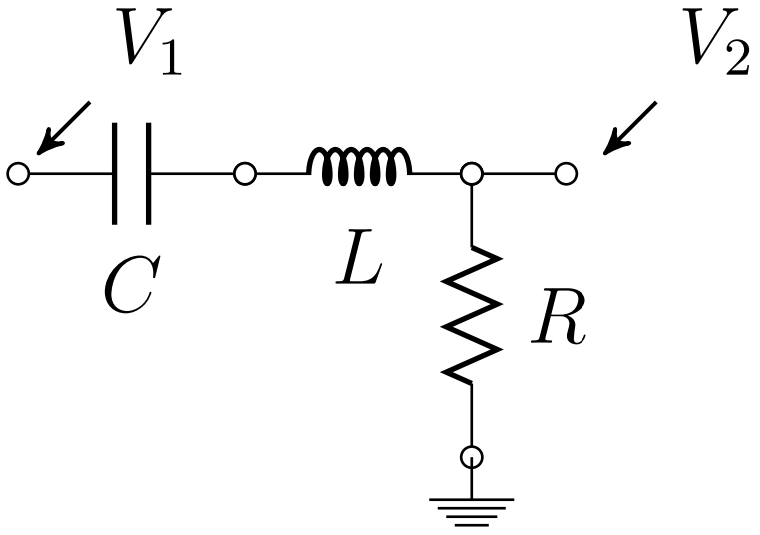
\includegraphics[scale=0.15]{FIGURARLC.png}
    \caption{Diagrama de um circuito RLC ressonante.}
    \label{FIGURA RLC}
    \end{figure}
    
    Então, foi montado um circuito RLC, como descrito na figura \cref{FIGURA RLC} com um capacitor de $C=24 \mu F$ medindo-se com o uso do osciloscópio a tensão no resistor de $R=150\Omega$ e a tensão de alimentação do circuito, fornecida pelo gerador de função. O gerador foi ligado na forma de onda senoidal, com uma tensão baixa (na faixa de $V_{in}=500mV$) e o osciloscópio ajustado para mostrar a forma XY, comparando a fase da tensão de entrada ($V_1$) com a da medida no resistor ($V_2$).
	
	A imagem obtida no osciloscópio é chamada de \textit{Figura de Lissajous} e o seu formato é alterado conforme se altera a diferença de fase entre as medidas dos dois canais. Essa defasagem decorre da presença do capacitor e do indutor no circuito, sendo que eles têm efeitos contrários na fase resultante. Desse modo, quando o capacitor compensa o efeito do indutor, o que caracteriza a ressonância, a diferença de fase entre ($V_1$) e ($V_2$) é nula e a figura representada é a reta bissetriz dos quadrantes ímpares. Desse modo, sabendo-se a capacitância nominal C, pode-se determinar a indutância L ou mesmo determinar frequência natural de ressonância do circuito. A frequência $f_o$ pode ser descrita como:

	\begin{equation}
        f_o = \dfrac{1}{2 \pi \sqrt{LC}}
	\label{fresson}
	\end{equation}

	Assim, variando-se a frequência através do gerador de função, até que a \textit{Figura de Lissajous} torne-se uma reta, é possível encontrar o valor da indutância do indutor e a frequência de ressonância.

	Essa parte do experimento foi repetida para cada um dos indutores utilizados.
	
	\begin{equation}
	    V_L = \dfrac{d \phi _B}{dt} = L \dfrac{di}{dt}
	    \label{TensaoIndutor}
	\end{equation}
	
	\begin{equation}
	    \phi _B = BA = Li
	    \label{FluxoMagnetico}
	\end{equation}
	
	Onde $V_L$ é a tensão no indutor, $\phi _B$ é o fluxo magnético, L é a indutância, i é a corrente, B é o campo magnético, e A é a área atravessada por ele.
	
	Da \cref{TensaoIndutor}, podemos depreender que a tensão no indutor é proporcional à variação do fluxo magnético dentro dele.
	
	Da \cref{FluxoMagnetico}, podemos inferir que o fluxo magnético depende do campo magnético que existe através do indutor. Já o campo magnético dentro do solenoide depende da corrente através do indutor (i), do seu comprimento (l) e do seu número de voltas (N), como é descrito na equação:
	
	\begin{equation}
	    B = \mu _o \dfrac{N}{l} i
	    \label{CampoMag}
	\end{equation}
	
	Dentro de um transformador, formado por dois indutores conectados através do núcleo de ferro, o fluxo magnético em cada indutor depende do fluxo gerado pelo outro indutor. Sendo $B_1$ o campo magnético gerado pelo primeiro indutor, e $A_2$ a seção interna do segundo solenoide, é possível descrever o fluxo causado no indutor 2 pelo 1 como:
	
	\begin{equation}
	    \phi _{21}=\int \overrightarrow {B}_{1}\cdot d\overrightarrow {A} = N_2 B_1 \pi R_{1}^2 = \dfrac{\mu _o N_2 N_1}{l}\pi R^2 i_ 1 = Mi_1
	    \label{fluxo}
	\end{equation}
	
    Observa-se que nessa equação, a integral foi resolvida, e o valor de $B_1$ foi substituído na equação. O termo $\dfrac{\mu _o N_2 N_1}{l}\pi R^2$ é uma constante que é chamada de M (indutância mútua).
	
	Então no caso ideal, a tensão medida no solenoide primário do indutor nada mais é que o descrito na \cref{TensaoIndutor},
	E no secundário a mesma coisa. Portanto pode-se assumir que as duas tensões se relacionam através de:
	
	\begin{equation}
	    \dfrac{V_p}{V_s}=\dfrac{N_p}{N_s}
	    \label{RazaoTensao}
	\end{equation}
	
	Por exemplo, um transformador ideal com um solenoide de 1000 voltas e outro com 500 voltas, a tensão medida no primeiro é o dobro da segunda.
	
	Agora, para estudar o efeito da transformação de tensão, é necessário compreender o indutor utilizado, que é composto de dois indutores unidos por um núcleo de ferro. Num indutor ideal, a perda de energia no núcleo é nula, pois a histerese também é, e o fluxo magnético numa seção do núcleo é igual a outra seção de mesma área.
	
	O fluxo magnético dentro do transformador depende do número de espiras que existem no solenoide do indutor.

	Depois de encontradas as indutâncias, foi montado o circuito da \cref{Circ1} com o gerador de função a frequência aproximadamente de 50Hz e com a tensão de pico-a-pico limitada a 5V ($V_{pp}=5V$) e com o osciloscópio medindo a tensão aplicada no primeiro indutor ($N_p$) e a tensão que aparece no segundo ($N_s$).
	Na primeira montagem, foi feita de forma que $N_p < N_s$. Então, com os instrumentos ligados a um computador com \texttt{MATLab}, adquirimos os dados de uma varredura de tensão para observar a proporcionalidade expressa na \cref{RazaoTensao}.
	Esse procedimento doi repetido para o caso em que $N_p > N _s$.
	
	% ==================================
    % CIRCUITO 1 (Circ1)
    %
    \begin{figure}[!htb]
    \centering
    \includegraphics[scale=0.25]{Circ1.pdf}
    \caption{Diagrama do circuito do transformador com bobinas de $N_p$ voltas no primário e de $N_s$ voltas no secundário.}
    \label{Circ1}
    \end{figure}

	Com a montagem de $N_s < N_p$, foi feita uma medição qualitativa da função do núcleo de ferro no indutor. O circuito da \cref{Circ1} foi montado, mas com os indutores concatenados e desacoplados do núcleo de ferro, e depois foi observado o comportamento das tensões medidas em cada indutor através do osciloscópio quando o núcleo de ferro foi introduzido lentamente entre as bobinas dos indutores. O foco foi em perceber se a proporção \cref{RazaoTensao} foi sempre mantida.

	Depois de terminada essa parte, para compreensão do efeito da indução e da transformação da tensão, foi montado o circuito da \cref{Circ2} com $N_p < N_s$, usando resistores de resistências nominais $R_1 = 4.7\Omega$ e $R=100k\Omega$ e um capacitor com capacitância nominal $C=24\mu F$. Nesta parte do experimento, não foi utilizado o gerador de função, e sim a tomada disponível no laboratório, dessa forma a frequência de entrada de circuito era a frequência da tomada (que no caso era de aproximadamente $60Hz$), onde foi ligado um transformador que reduzia a tensão da tomada a $18V_{rms}$.
	
	% ==================================
    % CIRCUITO 2 (Circ2)
    %
    \begin{figure}[!htb]
    \centering
    \includegraphics[scale=0.25]{Circ2.pdf}
    \caption{Diagrama do circuito para observar o fenômeno da histerese.}
    \label{Circ2}
    \end{figure}

	Assim, com o circuito montado, o osciloscópio foi ligado no modo XY para observação da histerese do núcleo férrico.
	
	O sinal do canal 1, $V_x$ é proporcional ao campo magnético H , enquanto que no canal 2 $V_y$, é proporcional ao fluxo magnético B.

    A partir da figura obtida no osciloscópio, sabemos o valor máximo da queda de tensão. Assim, podemos calcular o valor da tensão no resistor $R_1$ $V_{rms}$, da corrente $i_{rms}$ e da resistência equivalente $R_{eq}$:
    
    \begin{equation}
	    V_{rms} = \dfrac{V_{max}}{\sqrt{2}}
	    \label{Vrms}
	\end{equation}
	
	\begin{equation}
	    I_{rms} = \dfrac{V_{rms}}{R_1}
	    \label{Irms}
	\end{equation}
	
	\begin{equation}
	    R_{eq} = \dfrac{P_d}{i_{rms}^2}
	    \label{Req}
	\end{equation}
	
	Sendo $P_d$ o valor da potência RMS dissipada no transformador.

	\begin{figure}[!htb]
    \centering
    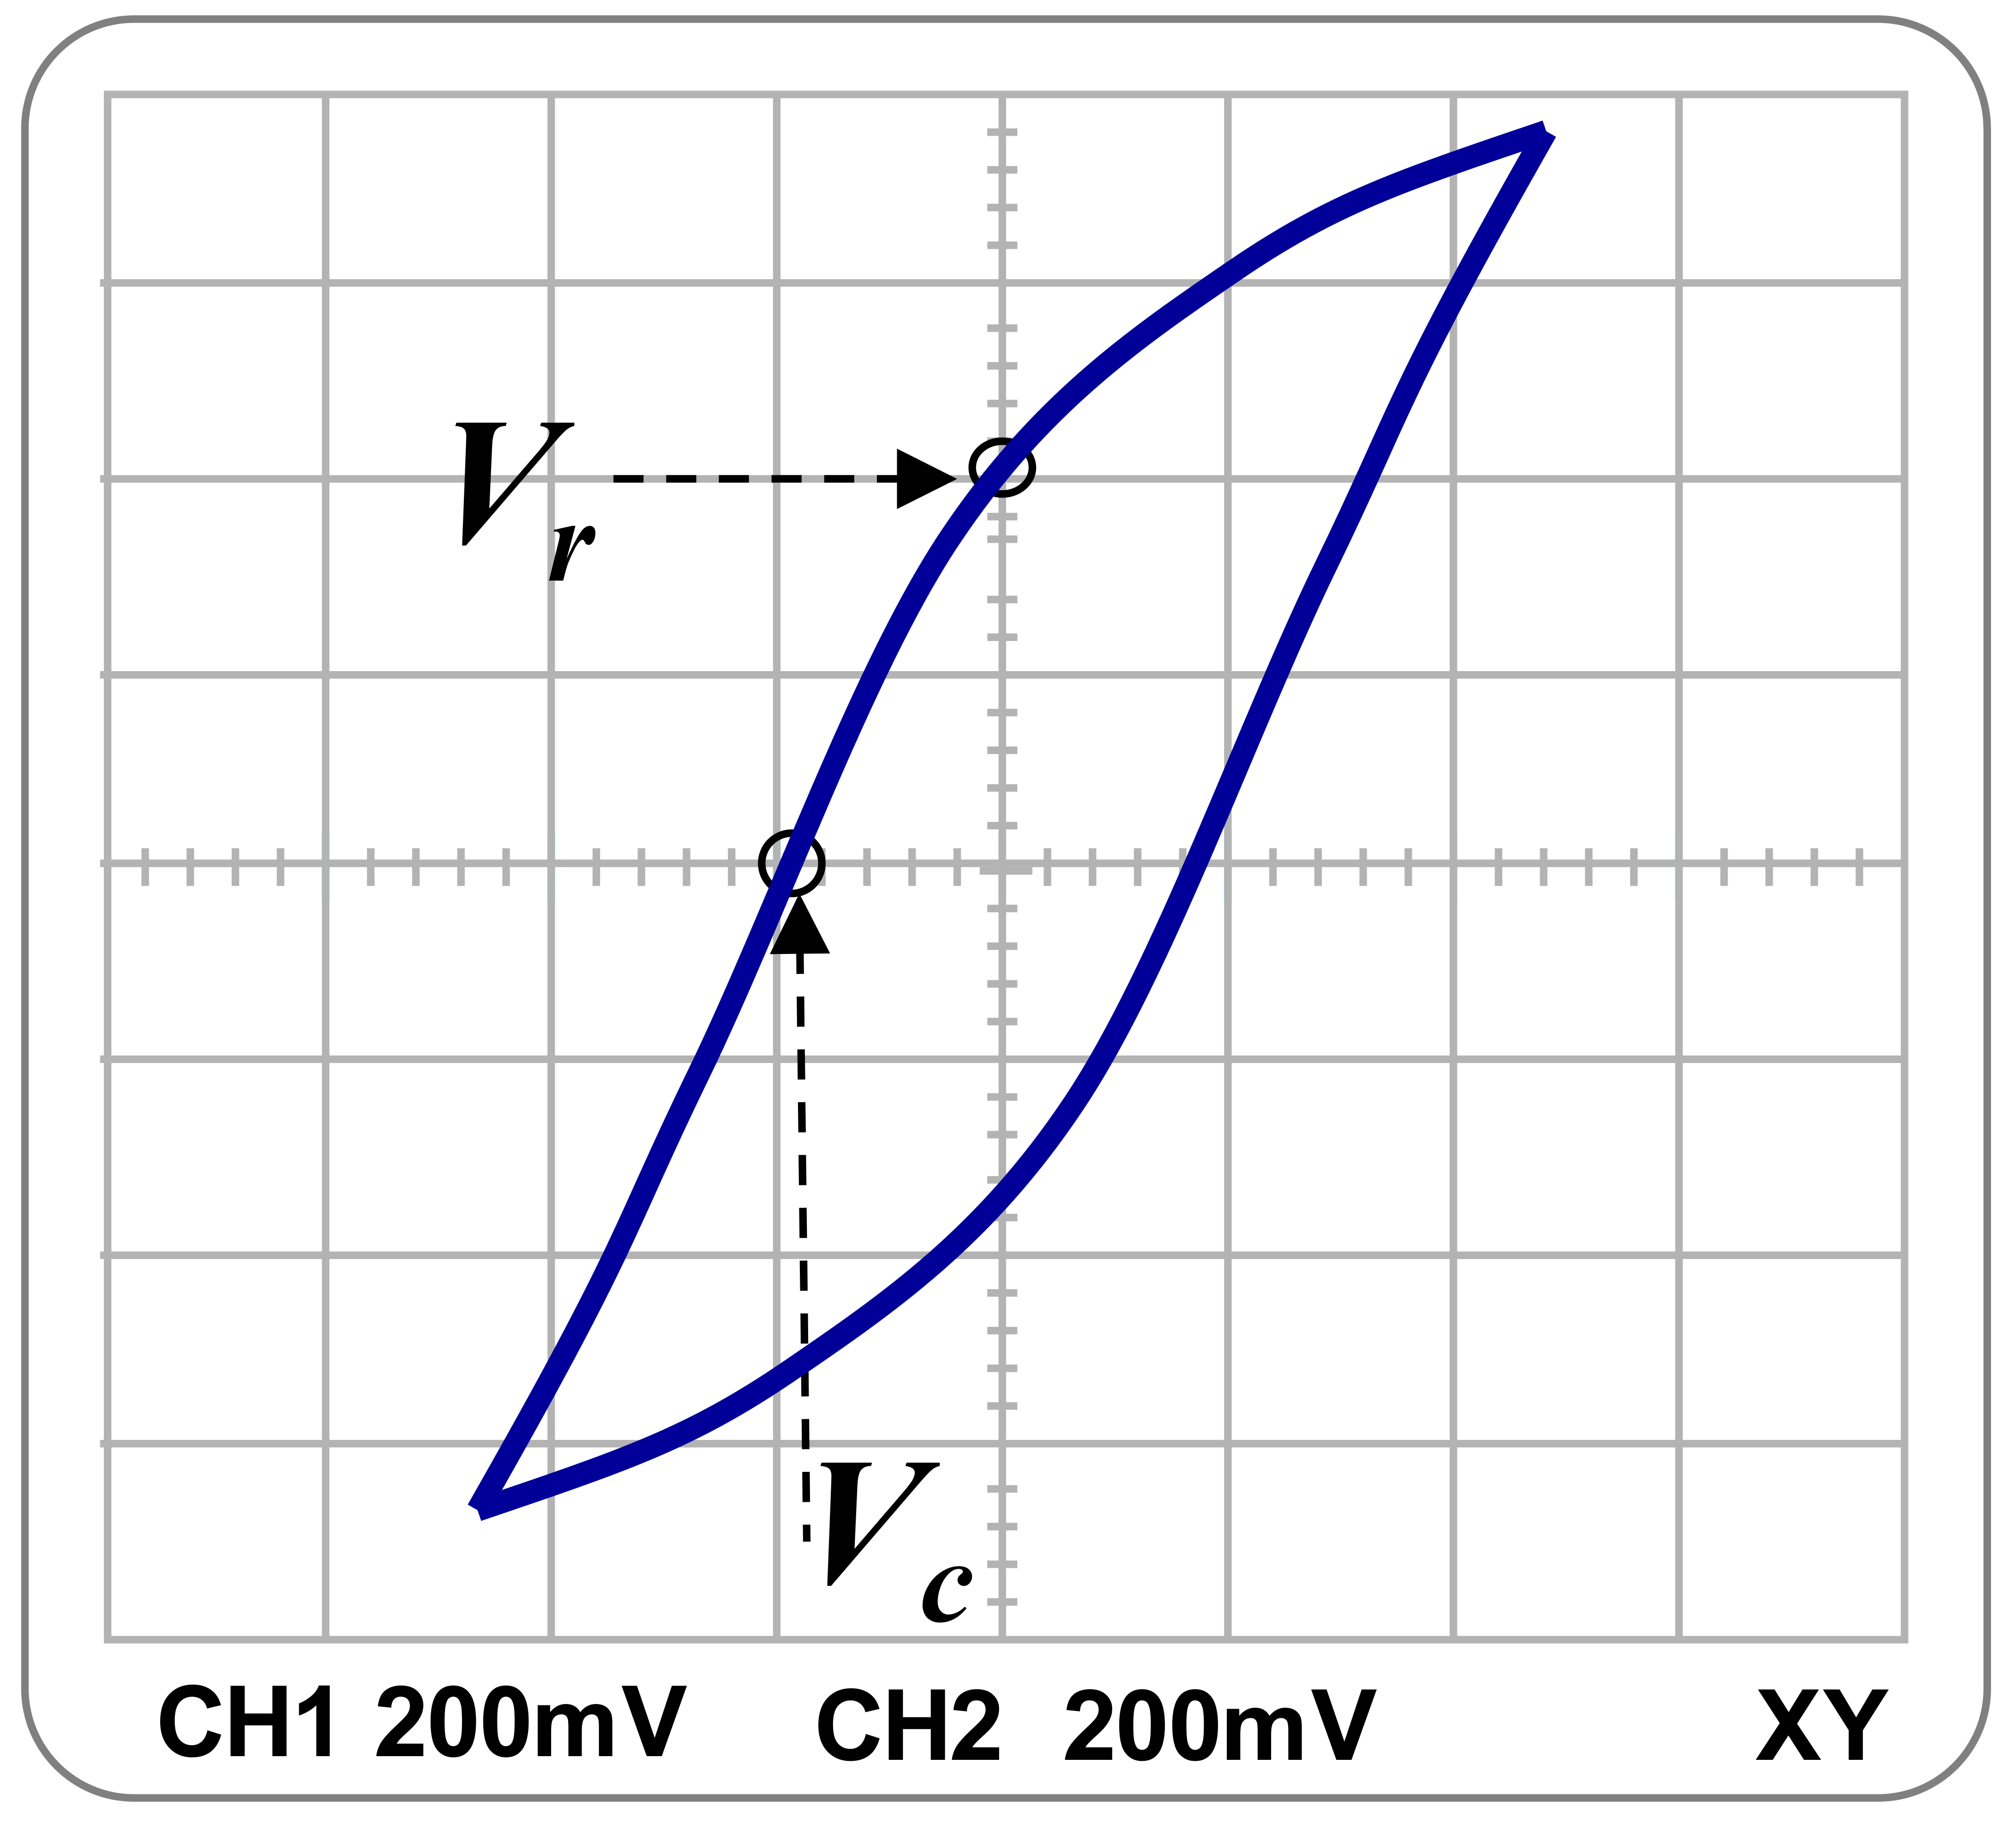
\includegraphics[scale=1.0]{Histerese.png}
    \caption{Figura típica de Lissajous para a histerese de um núcleo férrico.}
    \label{Histerese}
    \end{figure}

    Depois o osciloscópio foi alterado para o modo YT, e as formas de onda observadas foram capturadas com o auxilio do \texttt{MATLab}. A forma esperada era similar à \cref{Histerese}.
    
    Com a área da figura obtida, pudemos calcular a potência dissipada, $P_d$, que é definida por:
    
    \begin{equation}
        P_d = \dfrac{f R C N_p A}{R_1 N_s}.
        \label{Pot}
    \end{equation}
    
    A partir das tensões $V_r$ e $V_c$, indicadas na \cref{Histerese}, podemos calcular o valor do campo remanente $B_R$ e da força coercitiva $H_c$. A força coercitiva corresponde à tensão necessária para neutralizar o campo magnético da magnetização do núcleo, $V_c$, enquanto o campo remante corresponde à tensão que permanece devido à magnetização do núcleo, $V_r$.
    
	Com esses valores, podemos computar o valor do campo remanente $B_R$ e da força coercitiva através das equações:
	
	\begin{equation}
	    B_R = \dfrac{RCV_r}{SN_s}
	    \label{CampoR}
	\end{equation}
	
	\begin{equation}
	    H_c = \dfrac{N_p V_c}{R_1 L}
	    \label{ForcaC}
	\end{equation}
    
	Por fim, fizemos as medições das dimensões do núcleo de ferro utilizado no experimento, de forma que foi possível calcular o perímetro médio ($l$) e a área da seção transversal ($S$) usando as seguintes equações:
    
    \begin{equation}
	    l = 2(D - F) + 2(E-F)
	    \label{PerMedio}
	\end{equation}
	
    \begin{equation}
	    S = FB
	    \label{Area}
	\end{equation}
	
	Em que F, B, D e E são os valores das dimensões obtidos.
%
% ======================================
% RESULTADOS
%
\section{Resultados}
    Os valores eficazes dos componentes utilizados no experimento são: $V_x = (0.051 \pm 0.002) V$, $V_c = (-0.34 \pm 0.02) V$, $R = (98.8 \pm 0.1)\Omega$, $R_1 = (7.5 \pm 0.1) \Omega$ e $C = (28.12 \pm 0.01) \mu F$. As dimensões do núcleo do transformador, medidas com o auxílio de uma régua, são $F = (19.0 \pm 0.5)mm$, $B = (20.0 \pm 0.5)mm$, $D = (95.0 \pm 0.5)mm$ e $E = (72.0 \pm 0.5)mm$.
    
    \begin{figure}[!htb]
    \centering
    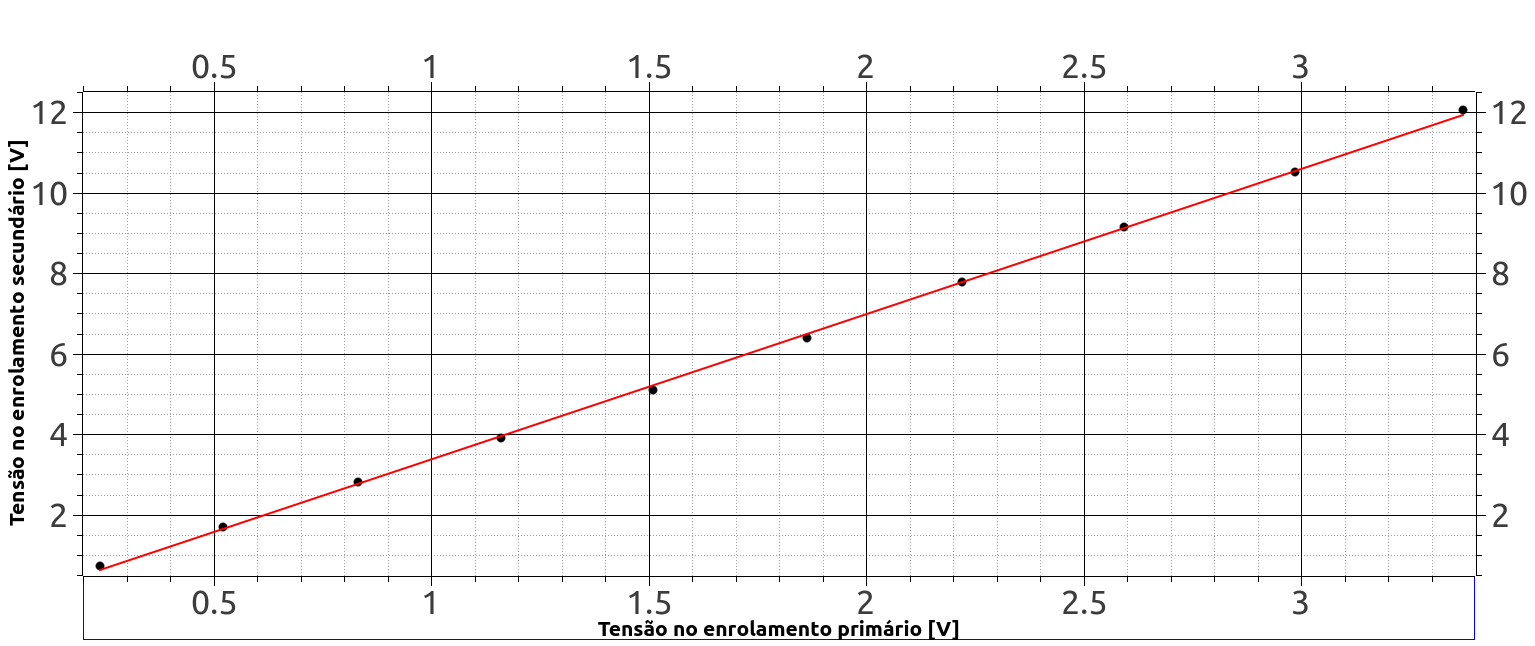
\includegraphics[scale=0.4]{Varredura2A.png}
    \caption{Gráfico obtido da Varredura em tensão comparando as tensões nos indutores 1 e 2 para Ns $>$ Np, de acordo com a montagem da \cref{Circ1}. A equação da regressão linear expressa em vermelho é $Y = (3.606 \pm 0.003)X - 0.23 \pm 0.05$. $\dfrac{Chi^2}{doF} = 0.0001575896$ $R^2 = 0.999557227$}
    \label{Varredura2A}
    \end{figure}
    
    \newpage
    \begin{figure}[!htb]
    \centering
    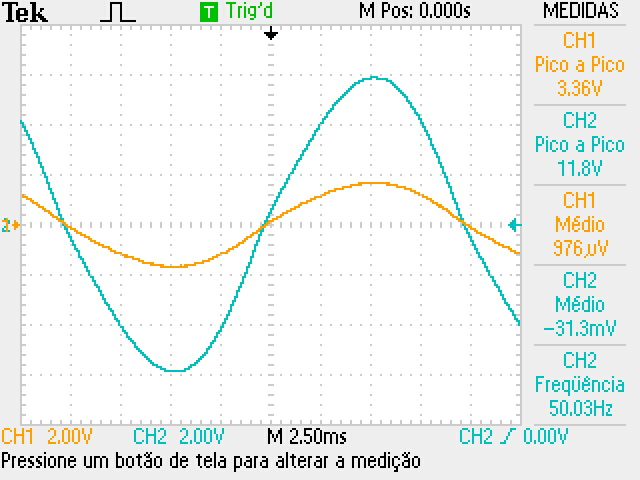
\includegraphics[scale=1]{FiguraA.JPG}
    \caption{Imagem da forma de onda obtida do osciloscópio varrendo o circuito da \cref{Circ1} para uma situação da \cref{Varredura2A}, onde $N_s < N_p$, ou seja, a tensão de saída é maior que a que entra no transformador. (Todas as legendas foram geradas automaticamente pelo osciloscópio.)}
    \label{FiguraA}
    \end{figure}
    
    \begin{figure}[!htb]
    \centering
    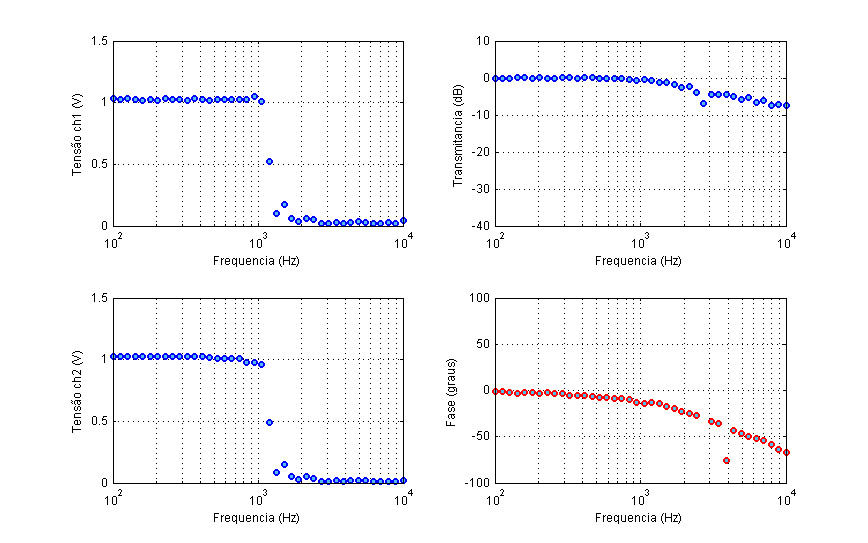
\includegraphics[scale=0.4]{Varredura2B.png}
    \caption{Gráfico obtido da varredura em tensão comparando as tensões nos indutores 1 e 2 para Ns $<$ Np, de acordo com a montagem da \cref{Circ1} A equação da regressão linear expressa em vermelho é $Y = (0.210 \pm 0.002)X - 0.019 \pm 0.006$. $\dfrac{Chi^2}{doF} = 7.344391$ $R^2 = 0.99935213017$}.
    \label{Varredura2B}
    \end{figure}
    
    \newpage
    \begin{figure}[!htb]
    \centering
    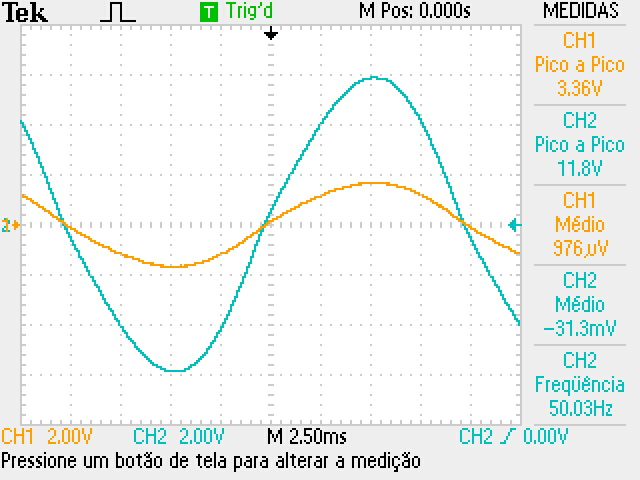
\includegraphics[scale=1]{FiguraA.JPG}
    \caption{Imagem da forma de onda obtida do osciloscópio varrendo o circuito da \cref{Circ1} para uma situação da \cref{Varredura2A}, onde $N_s > N_p$, ou seja, a tensão de saída é menor que a que entra no transformador. (Todas as legendas foram geradas automaticamente pelo osciloscópio.)}
    \label{FiguraB}
    \end{figure}
    
    \begin{figure}[!htb]
    \centering
    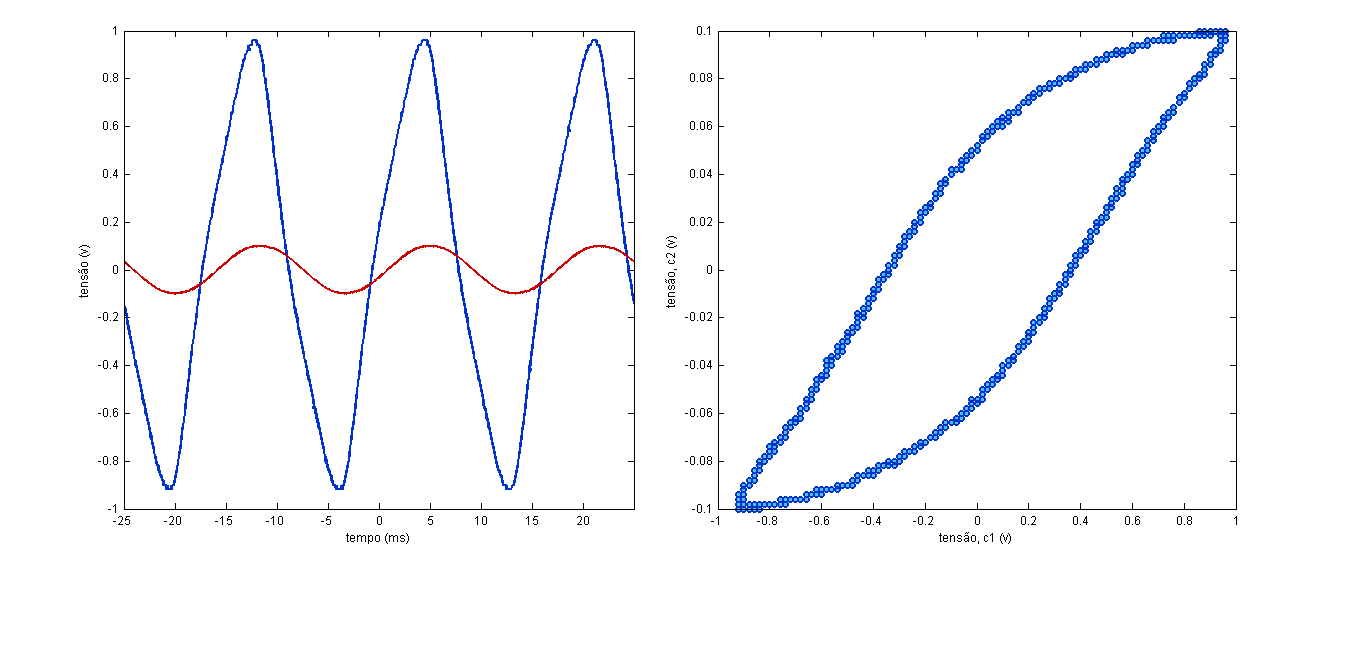
\includegraphics[scale=0.55]{Varredura3.png}
    \caption{Gráfico obtido através da figura obtida pelo \texttt{MATLab} da figura de \textit{Lissajous} representando a histerese decorrente da montagem da \cref{Circ2}.\newline A área interna ao segundo gráfico, da histerese, foi calculada por integração numérica em C++ e tem valor $(0.1195 \pm 0.0002)V^2$}
    \label{Varredura3}
    \end{figure}
%
% ======================================
% ANALISE DE DADOS
%
\newpage
\section{Análise de Dados}
    
    \subsection{Medidas de Indutâncias}
    %===================================
    % ITEM ROTEIRO 1
    Através da montagem do circuito da \cref{FIGURA RLC}, e medindo a tensão com o auxílio do osciloscópio, foi possível encontrar o valor das indutâncias reais dos indutores utilizados, colocando o osciloscópio no modo XY e ajustando a frequência de entrada de forma que a imagem observada se tornasse uma reta. Isso garantiria que o circuito havia entrado no estado de ressonância, e a frequência pode ser descrita através da \cref{fresson}, sabendo-se a frequência e a capacitância do circuito, isso permitia encontrar o valor da indutância.
    
    Para o primeiro indutor (que possuía menor número de espiras), a frequência de ressonância foi de $f_o = (50 \pm 1)10^{1}Hz$, como o capacitor utilizado tinha capacitância de $C= 28.12 \pm 0.01 \mu F$, a indutância pode ser calculada como sendo:
    \begin{gather*}
    f_{o}= \dfrac{1}{2 \pi \sqrt{LC}} \Rightarrow L= \dfrac{1}{4 \pi ^2 C f_0 ^2} \Rightarrow L_1= (3.6 \pm 0.1)mH
    \end{gather*}
    
    Para o segundo indutor (com maior número de espiras), o cálculo é análogo ao do indutor menor, para esse caso, a frequência de ressonância encontrada foi de $f_o = 128 \pm 1 Hz$. Assim o valor de indutância encontrado foi de:
    \begin{gather*}
    L_2=(55.0 \pm 0.9)mH
    \end{gather*}
    
    %==================================
    % ITEM ROTEIRO 2
    Depois, a mesma montagem da \cref{FIGURA RLC} foi feita para o indutor 1 (com menor número de espiras), mas dessa vez, ele foi introduzido ao núcleo férrico (que é utilizado para montagem do transformador). Pelo método das figuras de \textit{Lissajous}, a nova frequência de ressonância encontrada foi de $f_o=(110 \pm 1 HZ)$. Calculando-se a nova indutância do componente através da \cref{fresson}, foi possível encontrar a nova indutância como sendo:
    \begin{gather*}
        L_{nucleo}=(74.4 \pm 0.9)mH
    \end{gather*}
    
    \subsection{Ganho de Tensão no Transformador}
    
    %==================================
    % EM CASA ITEM 1
    
    Através do experimento feito com os circuitos montados da \cref{Circ1} foi possível obter os gráficos da \cref{Varredura2A} e \cref{Varredura2B}.
    
    Essas imagens representam a relação da tensão no primeiro indutor e no segundo. 
    É possível notar que a razão entre as tensões é aproximadamente constante, por isso a curva pode ser descrita através de uma função linear nos dois casos.
    
    Na \cref{Varredura2A}, onde $N_s < N_p$, a razão $|V_s / V_p|=3.606 \pm 0.003$, ou seja, houve um ganho de tensão de 3.606 vezes no transformador.
    
    Na \cref{Varredura2B}, onde $N_s > N_p$, a razão $|V_s / V_p|=0.210 \pm 0.002$, ou seja, houve uma perda de tensão de 0.21 vezes da tensão de entrada ao passar pelo transformador.
    
    A razão entre as tensões, ou seja, o ganho de tensão no transformador, pode ser descrito através da \cref{RazaoTensao}. Como o indutor 1 possui 400 espiras, e o indutor 2 cerca de 1600 espiras, a razão esperada pode ser calculada como:
    \begin{gather*}
        \dfrac{V_s}{V_p}=\dfrac{N_s}{N_p}=1600/400=4
    \end{gather*}
    
    
    \subsection{Histerese do Transformador}
    % ==================================
    % ITEM ROTEIRO 3 D
    %
    A fim de estudar o efeito da histerese do transformador, é importante ter uma análise do transformador em si, principalmente da sua forma, que influencia nesse efeito. A partir das dimensões medidas do núcleo do transformador, pudemos calcular o perímetro médio que percorrem as linhas de campo dentro do núcleo (l) usando a \cref{PerMedio}:
    \begin{gather*}
        (l \pm \Delta l) = (258 \pm 2)mm
    \end{gather*}
    
    E a área de seção transversal (S) usando a \cref{Area}:
    \begin{gather*}
        (S \pm \Delta S) = (38 \pm 1) 10 mm^2
    \end{gather*}
 
    % ==================================
    % EM CASA ITEM 2
    %
    
    Assim, como agora temos o valor de S, podemos substituir os valores calculados na \cref{CampoR} e computar o valor do campo remanente ($B_R$):
    \begin{gather*}
        (B_R \pm \Delta B_R) = (0.23 \pm 0.02)T
    \end{gather*}
        
    E calcular a força coercitiva ($H_c$) usando a \cref{ForcaC}:
    \begin{gather*}
        (H_c \pm \Delta H_c) = (-70 \pm 4) A/m
    \end{gather*}
    
    Essa força é o que representa a tendência do material férrico de manter as suas porpriedades anteriores (a histerese).
    
    
    
    %
    % =======================================
    % PARA CASA ITEM 3
    Para o cálculo da potência dissipada, primeiramente, calculamos a área $A$ da curva de histerese por integração numérica, (representada à direita da \cref{Varredura3}) e obtivemos:
    %
    \begin{gather*}
        A = (0.1195 \pm 0.0002)V^2
    \end{gather*}
    
    Assim, sabendo que a frequência da histerese é de $ f = (60.047 \pm 0.001) Hz $, $N_p = 400$ e $N_s = 1600$, substituímos esses valores na \cref{Pot} e obtemos que a potência dissipada no ciclo é:
    %
    \begin{gather*}
        (P_d \pm \Delta P_d) = (0.66 \pm 0.01)W
    \end{gather*}
    
    Pela curva capturada no resistor de $4.7 \Omega$ (representada à esquerda da \cref{Varredura3}), sabemos que a queda de tensão máxima foi de $V_{max}$. Assim, obtemos o valor de $V_{rms}$ a partir da \cref{Vrms} e, usando a \cref{Irms} podemos calcular o valor de $i_{rms}$ e, então, obter o valor da resistência equivalente $R_{eq}$ associada ao circuito, por meio da \cref{Req} .
    %
    \begin{gather*}
        (V_{max} \pm \Delta V_{max}) = (0.94 \pm 0.02)V\\
        V_{rms} \pm \Delta V_{rms} = (0.66 \pm 0.01)V\\
        (I_{rms} \pm \Delta I_{rms}) = (0.089 \pm 0.001) A\\
        (R_{eq} \pm \Delta R_{eq}) = (85 \pm 3)\Omega
    \end{gather*}

% ======================================
% ======================================
% DISCUSSAO
%
\section{Discussão}

    %% DISCUSSAO PARTE 1 E 2
    Da primeira parte do experimento, de medição das indutâncias dos indutores utilizados, foi encontrada a indutância do indutor 1 (de menor número de espiras) como $L_1=(3.6 \pm 0.1)mH$ e do indutor 2 como $L_2=(55 \pm 0.9)mH$. Esses valores estão bem próximos dos valores indicados nos próprios indutores, o indutor 1 tinha como valor nominal $L_{01}=(3.60 \pm 0.01)mH$ e o indutor 2 $L_{02}=(54.36 \pm 0.01)mH$, de fato, os valores se abrangem dentro das suas faixas de erro, isso condiz que essa parte do experimento foi feita corretamente. Todavia, os valores obtidos experimentalmente têm um erro associado maior que os valores nominais, isso se deve principalmente pelo método utilizado que associava um erro significativo à frequência de ressonância encontrada.
    Depois, a indutância foi calculada novamente para o indutor 1, mas dessa vez com o núcleo de ferro associado ao indutor, e houve um aumento significativo da indutância para $L_{nucleo}=(74.4 \pm 0.9)mH$. Esse aumento associado está de acordo com o esperado pela literatura, já que o valor do $\mu$ (a permeabilidade magnética do meio) para o ferro é bem maior que o do ar. Podemos observar através da \cref{CampoMag} que o campo magnético gerado pelo indutor (que é diretamente proporcional à sua indutância) depende de $\mu$, então a indutância deveria mesmo aumentar ao adicionar o núcleo de ferro.
    
    %%Discussao PARTE CASA 1
    Quando observamos o comportamento descrito pelas \cref{Varredura2A} e \cref{Varredura2B}, foi possível encontrar o ganho de tensão no transformador utilizando os indutores de indutância calculada anteriormente como sendo de $(3.606 \pm 0.003)$. O ganho de tensão teve um comportamento linear com a variação da tensão, assim como esperado através da \cref{RazaoTensao}, a razão é uma constante. Todavia, como o número de espiras do indutor 1 é de 400 espiras, e do indutor 2 de 1600 espiras, a razão $\dfrac{V_s}{V_p}=\dfrac{N_p}{N_s}$ deveria valer 4. Essa diferença se deve ao fato que o transformador não é ideal, ele possui uma resistência interna que não é nula, e a própria histerese do núcleo afeta a proporção de tensão. 
    É interessante notar que o inverso do coeficiente angular do \cref{Varredura2A} ($a^{-1}_1=1/3.06 \Rightarrow a^{-1}_1 = 0.28 \pm 0.02$) quando somado ao coeficiente angular do \cref{Varredura2B} ($0.0.21 \pm 0.02$), para o qual a ordem dos enrolamentos foi invertida corresponde à $0.49 \pm 0.03$ que é próximo de 0.5, o que seria esperado para 2 vezes 0.25 que deveria ser o valor obtido do segundo coeficiente. Isso significa que embora haja um desvio no inverso do primeiro coeficiente e no segundo coeficiente em relação à razão do número de espiras dos indutores, estes estão aproximadamente a mesma distância do valor esperado, o que indica que a caus dos desvios é a mesmo nos dois casos que é o fato do transformador não ser ideal (o mesmo ocorre entre o inverso do segundo coeficiente quando somado ao primeiro). 

    Na última parte do experimento, calculamos os valores do campo remanente $B_R$ a partir da análise da tensão $V_Y$ na figura da histerese e dos valores conhecidos de R, C, S, e $N_S$. Calculamos também o valor da força coercitiva, $H_C$, com os valores conhecidos de $N_P$, $R_1$, e do período L.
    Os valores obtidos foram $B_R = (0.23 \pm 0.02)T$ e $H_C = (70 \pm 4)A/m$. Ambos os valores são razoáveis.
    
    Através do cálculo da área da figura da histerese $A = (0.1195 \pm 0.0002)V^2$, e com este valor, calculamos a potência dissipada no tranformador, $P_d = (0.66 \pm 0.01)W$.
    
    É interessante notar que a magnetização e desmagnetização do núcleo férrico tem um custo energético, que corresponde à $P_d$. Isso demonstra que o transformador de fato não é ideal, e essa análise pode ser extendida ao mundo real, em que transformação de tensão, em redes de distribuição de potência por exemplo, representam gastos significativos de energia.
    
    Com o valor da tensão RMS no resistor $R_1$, $V_{rms}$, obtivemos $I_{rms} = (0.089 \pm 0.001)A$. Então pudemos determinar a resistência equivalente do primeiro enrolamento do tranformador mais $R_1$, $R_{eq} = (85 \pm 3)\Omega.$
    
    Considerando a resistência nominal interna do indutor $I_1$, $R_i = (63.5 \pm 0.1)\Omega$, e $R_1 = (7.5 + 0.1)\Omega$, o valor obtido ($85 \pm 3) \Omega$ é bastante razoável.
    
    Um ponto importante que funcionou como fonte de erro para o experimento, era a instabilidade de acoplamento dos indutores ao núcleo de ferro, já que era difícil de garantir o alinhamento ideal dos solenoides e seu \textit{encaixe} no núcleo de ferro, além dos encaixes da \textit{Protoboard} e da resistência dos cabos utilizados que interferiam nos dados medidos do experimento.
    
    
% ======================================
% ======================================
% CONCLUSAO
%
\section{Conclusão}
    Nesse experimento, pudemos compreender a transformação da tensão em transformadores formados por bobinas acopladas através do núcleo de ferro e o fenômeno de histerese neste. 
    Foi possível encontrar experimentalmente através do método das figuras de \textit{Lissajous} o valor da indutância dos indutores como sendo (Indutor de 400 espiras) $L_1 = (3.6 \pm 0.1)mH$ e (Indutor de 1600 voltas) $(55.0 \pm 0.9)mH$ que são valores condizentes com os valores nominais dos indutores utilizados de ($3.60 \pm 0.01$)mH e ($54.36 \pm 0.01$mH), respectivamente.
    Pudemos observar o ganho de tensão num transformador na forma $N_p < N_s$, e que isso é proporcional à razão do número de espiras entre as bobinas do transformador de maneira constante.
    A curva obtida da histerese, pelo osciloscópio no modo XY, do núcleo de ferro teve o formato esperado que mostrava a tendência do material de conservar as suas propriedades magnéticas.
    O valor encontrado da resistência equivalente do circuito foi de $R_i=(85 \pm 3)\Omega$ foi dentro do esperado que condizia ao valor da soma das resistências do circuito.
    Dessa forma, o experimento realizado esteve coerente com o esperado pela literatura, e permitiu um estudo acerca do funcionamento de um transformador e da sua característica de histerese.
    


% ======================================
% ======================================
% INSTRUMENTOS UTILIZADOS
%
\newpage
\section{Instrumentos utilizados}
Os instrumentos utilizados neste experimento foram,
\begin{itemize}
	\item Osciloscópio Tektronix 10002B
	\item Gerador de funções arbitrárias BK Instruments 4052
	\item Multímetro DT830 Digital
\end{itemize}

%
% ======================================
% PROPAGACAO DE ERROS
%
\section{Propagação de erros \label{ap:erros}}
    \begin{enumerate}
        \item Erro da indutância calculada a partir da \cref{fresson}:\\
            $\Delta L = \sqrt{ \left (\dfrac{\Delta C}{4 \pi ^2 C^2 f_o^2} \right ) ^2+\left ( \dfrac{\Delta f_o}{2 \pi ^2 C f^3_o} \right ) ^2}$
        \item Erro do perímetro médio a partir da \cref{PerMedio}:\\
            $\Delta l = \sqrt{4\Delta F^2 + 4\Delta G^2}$
        \item Erro da área da seção transversal a partir da \cref{Area}:\\
            $\Delta S = \sqrt{B^2 \Delta F^2 + F^2 \Delta B^2}$
        \item Erro do campo remanente a partir da \cref{CampoR}:\\
            ${\Delta B_R^2} = {\left(\dfrac{\Delta R C V_R}{S N_S}\right)^2} + {\left(\dfrac{\Delta C R V_R}{S N_S}\right)^2} + {\left(\dfrac{\Delta V_R R C}{S N_S}\right)^2} + {\left(\dfrac{\Delta S N_S R C V_R}{S^2 N_S^2}\right)^2}$
        \item Erro da força coercitiva a partir da \cref{ForcaC}:\\
            ${\left(\dfrac{\Delta H_c}{ H_c}\right)^2} = {\left(\dfrac{\Delta R_1}{ R_1}\right)^2} + {\left(\dfrac{\Delta L }{ L}\right)^2} + {\left(\dfrac{\Delta V_C}{ V_C}\right)^2}$
        \item Erro da potência dissipada no ciclo a partir da \cref{Pot}:\\
            ${\left(\dfrac{\Delta P_d}{P_d}\right)^2} = {\left(\dfrac{\Delta f}{f}\right)^2} + {\left(\dfrac{\Delta C}{C}\right)^2} + {\left(\dfrac{\Delta R}{R}\right)^2} + {\left(\dfrac{\Delta A}{A}\right)^2} + {\left(\dfrac{\Delta R_1}{R_1}\right)^2}$
        \item Erro da tensão $V_{rms}$ a partir da \cref{Vrms}:\\
            $\Delta V_{rms} = \dfrac{\Delta V_{max}}{\sqrt{2}}$
        \item Erro da corrente $i_{rms}$ a partir da \cref{Irms}:\\
            $\Delta I_{rms} = \sqrt{{\left(\dfrac{\Delta V_{rms}}{R_1}\right)^2} + {\left(\dfrac{\Delta R_1 V_{rms}}{R_1^2}\right)^2}}$
        \item Erro da resistência equivalente a partir da \cref{Req}:\\
            $\Delta R_{eq} = \sqrt{{\left(\dfrac{\Delta P_d}{i_{rms}^2}\right)^2} + {\left(\dfrac{2 \Delta i_{rms} P_d}{i_{rms}^3}\right)^2}}$
            
    \end{enumerate}


\newpage
%
% ======================================
% REFERENCIAS
%
\begin{thebibliography}{10}

\bibitem{apostila}Gustavo Wiederhecker e colaboradores, \textsl{Roteiros de F429 - Corrente alternada e óptica.} Compilado em 26 de setembro de 2016.

\bibitem{livro texto}[Boyce and DiPrima, 2009 Boyce, W. E. and DiPrima, R. C. (2009)]. Elementary differential equations and boundary value problems. Wiley, Hoboken, NJ, 9th ed edition.

\bibitem{livro}[Yaro Burian Jr. e Ana Cristina Lyra]. Circuitos Elétricos.

\bibitem{livro2}Fundamentos da Física, Volume 3 - $9^a$edição.

\end{thebibliography}

\end{document}